\documentclass[12pt]{article}

\usepackage{amsfonts}
\usepackage{graphicx}
\usepackage{float}
\usepackage{titling}

\setlength{\droptitle}{-10em} 
\addtolength{\oddsidemargin}{-.875in}
\addtolength{\evensidemargin}{-.875in}
\addtolength{\textwidth}{1.75in}
%\addtolength{\textheight}{1.75in}

\begin{document}
	
	\title{Networks:  Replication Assignment} 
	
	\author{Cindy Cook}
	\date{15 March 2016}
	\maketitle
	\vspace{-12mm}

\section{Introduction}

The paper, ``High-Reproducibility and High-Accuracy Method for Automated Topic Classification," consists of four main parts \cite{main}. The first points out a major limitation to the LDA algorithm developed by Blei as a topic model \cite{lda}. The second describes a new method called TopicMapping developed to overcome theoretical drawbacks of LDA. The third consists of comparing the accuracy and reproducibility of TopicMapping as compared to LDA and pLSA \cite{plsa} on synthetic data. The final aspect of the paper, applies TopicMapping to two real world datasets. This paper aims to reproduce and extend these results. In particular, I will focus on reproducing only accuracy and reproducibility results for the comparisons between TopicMapping and randomly seeded LDA.     

\section{Replication}
\subsection{LDA Limitations}

The paper \cite{main} begins with a simple thought experiment. Given a Corpus consisting of documents in three distinct languages, say English, Spanish, and French, let all words in each language be unique and each document contain only one language. Ideally, a topic model would produce three distinct topics, one for each of the unique languages. However, this is not the case with LDA. The authors of \cite{main} show the likelihood of the generative model (i.e. placing all English documents in one topic, all Spanish documents in another, and all French documents in the last topic) is not always maximum. In fact they describe an alternative model, which theoretically obtains a higher likelihood. The alternative model is defined by separating one language into two dialect topics and combining the other two languages into one topic. In fact the authors prove in the supplemental material that, ``it is possible to find an extremely large number of alternative models (with the same number of topics) which overfit some topics and underfit some others but have a better likelihood then the true generative model" \cite{mainExtra}. These results are visualized in Fig. 2 (pg. 3,\cite{main}). Part a illustrates the differences in the generative and alternative models considered. Part b and c show the theoretical limits on the log likelihood for both generative and alternative models when considering a vocabulary of $60$ unique words, where $20$ are in either $E, S,$ or $F$. The corpus contains $1000$ documents, where each document contains $10$ words chosen uniformly from one language. Specifically, they show that the for these particular parameter values, if the fraction of $E$ documents in the corpus is greater than $0.936,$ then the likelihood of the alternative model become greater than the likelihood for the generative model. 
\\

\noindent In order to replicate part d of Fig. 2, I will first create a synthetic language corpus and then apply the LDA algorithm as programed in the \textit{topicmodels} package in R. We can determine the success rate as shown in Fig. 2 (pg. 3 \cite{main}) part d. Here, I also consider the average cosine similarity between each document's topic distribution and the true topic distribution. Following the process in \cite{main}, I first create a list of twenty words in English $E$, Spanish $S$, and French $F$. I then create a corpus of $1000$ documents, where the number of $E, S,$ and $F$ documents follow the following equation:
$$
100=pE+\frac{(100-p)}{2}S+\frac{(100-p)}{2}F,
$$ 
for $p=0.5, 0.6, 0.7, 0.8, 0.9, 0.96$. Note that each of the twenty words of a particular language has an equal probability of being sampled for each document with replacement, and each document consists of exactly ten words. I then apply LDA using the Variational EM Approach, which was used in \cite{main}. I run the algorithm $100$ times calculating the average cosine similarity and success rate with each run to obtain the following results:   
	\vspace{2mm}
	\begin{center}
		\begin{tabular}{ ||c|c|c|c|c|c|c||  }
			\hline
	          $p$ &0.5&0.6&0.7&0.8&0.9&0.96 \\ 
	         \hline 
          Min.    &0.5763 &0.5593 &0.5318 &0.5780 &0.5774 &0.5765\\
          1st Qu. &0.5844 &0.5821 &0.5802 &0.5800 &0.5791 &0.5774\\
          Median  &1.0000 &0.5871 &0.5834 &0.5822 &0.5802 &0.5777\\
          Mean    &0.8252 &0.7240 &0.6481 &0.5919 &0.5803 &0.5776\\
          3rd Qu. &1.0000 &1.0000 &0.5913 &0.5852 &0.5809 &0.5779\\
          Max.    &1.0000 &1.0000 &1.0000 &1.0000 &0.5858 &0.5783\\
          \hline
          \end{tabular}
        \end{center}
        \vspace{2mm}

\noindent We Notice that the minimum cosine similarity stays relatively constant across percent levels. This is due to the fact that in all runs, there are only three options of outcomes:  First, LDA correctly identifies the generative model resulting in a cosine similarity measure of about $0.99$; Second, LDA identifies the alternative model resulting in a cosine similarity of about $0.73$; and Third, LDA assigns a uniform topic distribution for each document resulting in a cosine similarity of about $0.55$. Although LDA applies a uniform topic distribution each of the corpuses at least once, we notice that when the percent level is $0.9$ and $0.96$ the algorithm applies a uniform topic distribution in all $100$ runs. Also, notice that the average cosine similarity decreases as the percent of English documents increases as expected. The following plot shows the success rate as the percentage of runs that correctly identifies the generative model:  
\begin{center}
	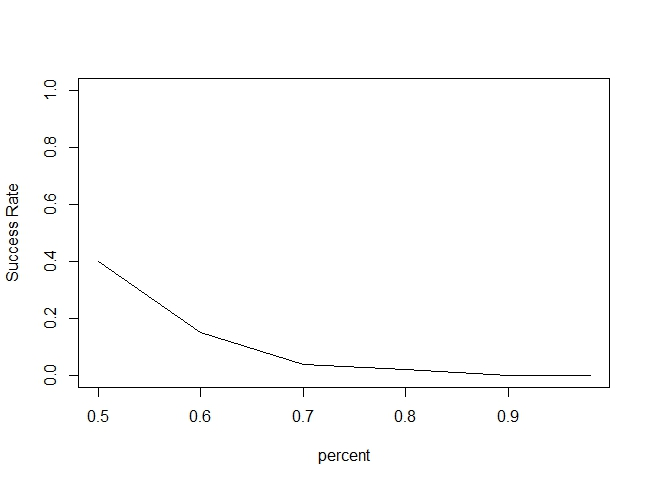
\includegraphics[scale=0.5]{Images/plot_smallC.jpeg}
\end{center} 
\vspace{2mm}
We now notice that the success rate is lower than the paper suggests, but there are many reasons for this. First, we are not analyzing the same corpus. Second, LDA uses Variational EM methods to fit the topic distribution, which is a stochastic process. Even though the overall success rate is lower, the trend stays the same. LDA tends to produce the correct generative model when the percentage of English documents is lower. In this example, when the percentage of English documents is greater than $0.9$, LDA never produces the generative model.

\subsection{TopicMapping}

The second part of the paper introduces a new algorithm for topic modeling called TopicMapping. The algorithm is described in \cite{main}, with more details in \cite{mainExtra}. In order to reproduce the article's main empirical results, I need to run their algorithm. I contacted the author's to not only obtain their original data, but their code if possible. I received code from one of the authors. The code is written mostly in C++, but also in Python. After several attempts, I was able to successfully run their code on a mac, but have run into the following error on a pc:  ``InfoMap did not compile. Please contact me: arg.lanci@gmail.com ." I have sent an email asking for help, but have yet to hear back. I was also able to code the algorithm in R. However, my code is neither efficient nor fast. For the following results, I ran everything I could on my pc, but decided to simply run the TopicMapping algorithm on a mac, save the results to a flash drive, and upload them to my pc for analysis. 

\subsection{Comparison of LDA to TopicMapping}

There are two types of major synthetic data analyzed in the paper. The first type of data is similar to that in Section 2.1, with corpuses of differing sizes contain ten languages in different proportions. The other type of data consists of corpuses constructed using the generative process defined in \cite{lda}, where the number of documents is $1000,$ the number of words in each document is $50$, the number of topics is set to $20$, and the hyper-parameters are set at $\alpha=0.001,0.004,0.016,0.064$. They also vary the percentage of words in the corpus that are considered generic, or equally likely across topics. Along with considering cases where each topic is equally distributed across documents, they consider cases where four topics make up $15\%$ and the last $16$ topics make up $2.5\%$. To simplify the amount of computing, I will focus on six corpuses of the first type:  Three corpuses have ten equally distributed languages of size $1000, 5000, 10000,$ and the other three have two languages making up $15\%$ each of the corpus and the remaining eight languages making up $8.75\%$ of size $1000, 5000, 10000$. I will also analyze twelve corpuses of the second type:  Six corpuses have $\alpha=0.001$ with generic proportion $0.2, 0.5, 0.8,$ and either equal topic distribution or not; the last six have $\alpha=0.064$ with generic proportion $0.2, 0.5, 0.8$, and either equal topic distribution or not.
\\

\noindent I was able to compile the code given to me by the authors, which simulate similar, but not the exact synthetic datasets. They did not save their original seed values. I was also able to successfully compile their program, which calculates the accuracy and reproducibility of a model. My aim is to reproduce the results as shown in Fig. 4 (pg.5, \cite{main}) and Fig. 7 (pg.6, \cite{main}) using a mac to run the TopicMapping algorithm and my pc to run LDA in R. The two other models that are considered by the authors are pLSA and LDA with seeded start values. Since the authors do not provide an explanation of what the start seeds are or how to find them, I ignore this model comparison. I also ignore the comparison to pLSA since this algorithm is not already programed in R nor do the authors provide code for it. The results for LDA and pLSA were similar to the results of LDA in all cases studies considered. Therefore, I will focus on reproducing the results for comparisons between TopicMapping and randomly seeded symmetric LDA only.
\\

\noindent I begin with the language corpuses, where I obtained the following accuracy and reproducibility results:
\vspace{2mm}
\begin{center}
	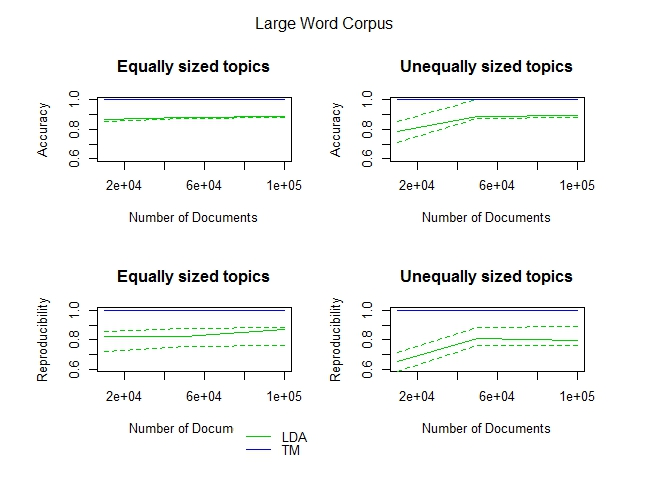
\includegraphics[scale=0.8]{Images/plot_largeC.jpeg}
\end{center} 
\vspace{2mm}
\noindent The plot above shows accuracy (top) and reproducibility (bottom) results for running LDA (green) and TopicMapping (blue) $100$ times on both equal (left) and unequal (right) topic distributions. With both algorithms, the number of topics was fixed at $10$. The median for the $100$ runs is plotted, where dotted lines indicate the $25$th and $75$th percentiles for both algorithms as described in \cite{main}. We can clearly see that the results follow the same patterns as shown in \cite{main}. TopicMapping is performing at near perfect accuracy and reproducibility for both equally and unequally sized topics regardless of the number of documents in the corpus. LDA clearly performs with greater variance, and does slightly better as the number of documents increases. Yet, TopicMapping outperforms LDA in all cases.
\\

\noindent The next results we will look at are those obtained from running both LDA and TopicMapping on the second set of simulated datasets when the hyper-parameters are set to $0.001$:
\vspace{2mm}
\begin{center}
	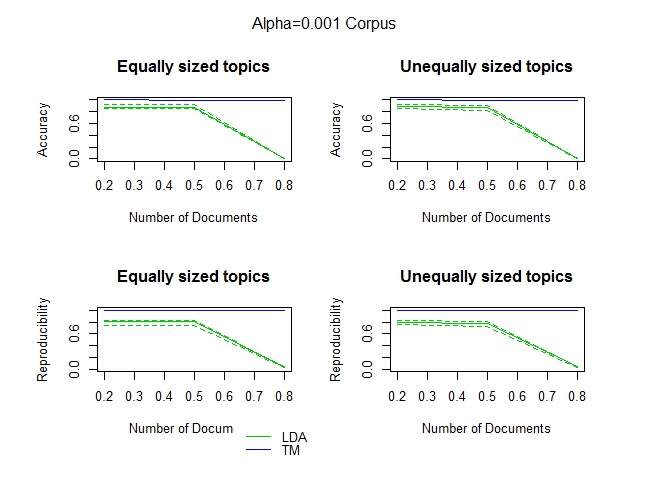
\includegraphics[scale=0.8]{Images/plot_Alpha1.jpeg}
\end{center} 
\vspace{2mm}

\noindent The figure above shows accuracy (top) and reproducibility (bottom) results for running LDA (green) and TopicMapping (blue) $100$ times on both equal (left) and unequal (right) topic distributions. With both algorithms, the number of topics was fixed at $20$ and the hyper-parameters are set at $0.001$. Again, the median for $100$ runs is plotted, where dotted lines indicate the $25$th and $75$th percentiles for both algorithms. We can clearly see that the results follow the same patterns as shown in \cite{main}. TopicMapping is performing at near perfect accuracy and reproducibility for both equally and unequally sized topics regardless of the number of documents in the corpus. LDA clearly performs with greater variance, and does slightly better as the percentage of generic words decreases. Yet, TopicMapping outperforms LDA in all cases.
\\

\noindent Lastly, we will look at the results obtained from running both LDA and TopicMapping on the second set of simulated datasets when the hyper-parameters are set to $0.064$:
\vspace{2mm}
\begin{center}
	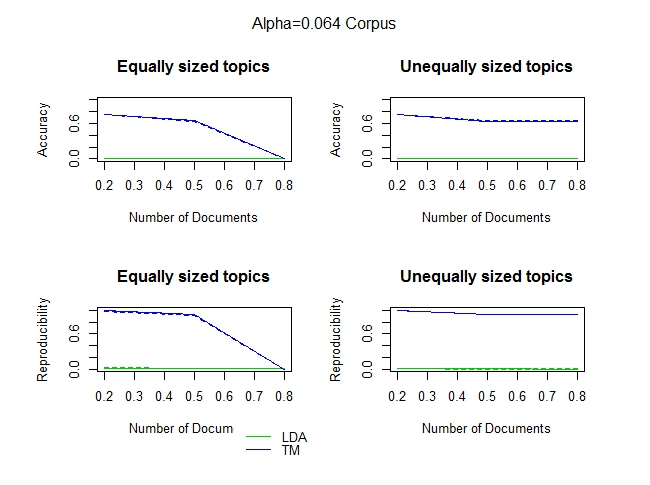
\includegraphics[scale=0.8]{Images/plot_Alpha2.jpeg}
\end{center} 
\vspace{2mm}

\noindent The figure above shows accuracy (top) and reproducibility (bottom) results for running LDA (green) and TopicMapping (blue) $100$ times on both equal (left) and unequal (right) topic distributions. With both algorithms, the number of topics was fixed at $20$ and the hyper-parameters are set at $0.064$. Again, the median for $100$ runs is plotted, where dotted lines indicate the $25$th and $75$th percentiles for both algorithms. We can clearly see that the results follow similar patterns as shown in \cite{main}. Both LDA and TopicMapping perform uniformly across differing percentages of generic words. TopicMapping with $0.7$ accuracy and $0.8$ reproducibility outperforms LDA, which performs poorly. Although LDA consistently performs poorly with unequally sized topics, TopicMapping's accuracy and reproducibility drop as the percentage of generic words increases, which is exactly what we see in \cite{main}.

   
\subsection{Applications}

I received emails back from two of the authors providing me with the corpus for the first application dataset:  \textit{Web of Science} or WoS. Both authors stated that the second application dataset, Wikipedia, was too large to send. They stated that even if they provided me access to it through some means, I would be unable to successfully reproduce their results in a semester. I will focus on reproducing the results for the first application only. The WoS Corpus contains documents consisting of the titles and abstracts for $23838$ journal articles published in six different top journals for the following fields:  astronomy, biology, economics, geology, mathematics, and psychology. I was able to reproduce the results on Fig. 8 (pg. 7, \cite{main}):

\vspace{2mm}
\begin{center}
	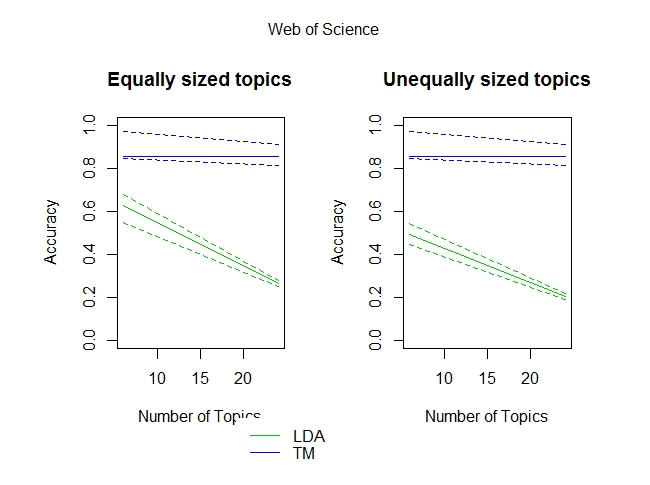
\includegraphics[scale=0.5]{Images/plot_WoS.jpeg}
\end{center} 
\vspace{2mm}  

\noindent I have plotted the median accuracy (left) and reproducibility (right) from the $100$ runs for both TopicMapping (blue) and LDA (green) with dotted lines representing the $25$th and $75$th percentiles. The results were found when the number of topics was set at $6$ the correct number and at $24$ as in \cite{main}. We notice that with both cases the correct number of topics and incorrect number, TopicMapping does well in both accuracy and reproducibility. However, LDA performs better when the correct number of topics specified. Again, TopicMapping outperforms LDA in all cases. 

\section{Extention}
\subsection{Creating the Network}
Due to the size of the WoS dataset, I am planning on randomly selecting $10$ documents in each subject to create a working dataset. After obtaining the $60$ randomly chosen documents, this network of words is created in R by first using the \textit{tm} package to obtain the term frequency matrix. The \textit{bipartite} package is then used to project this term frequency (i.e. the adjacency matrix for a two-mode network) onto a one-mode network of words. There are $2259$ unique words, which will become nodes in the network. Edges are created between words when the two words appear in the same document and are weighted by the number of times each pair of words appear in the same document. There are $167050$ edges. These weights have been shown to follow a Poisson distribution. Following the process laid out in \cite{mainExtra}, I keep only the statistically significant edges. The final network has $2259$ nodes and $166902$ edges. 
  
\subsection{Descriptive Statistics}
To begin analysis on this network, I use the \textit{igraph} package in R to measure the betweenness centrality for each node, which will allow me to analyze structural holes and bridges. Words that are highly used within each document and common across documents should have high betweenness scores.
 
%\vspace{2mm}
%\begin{center}%	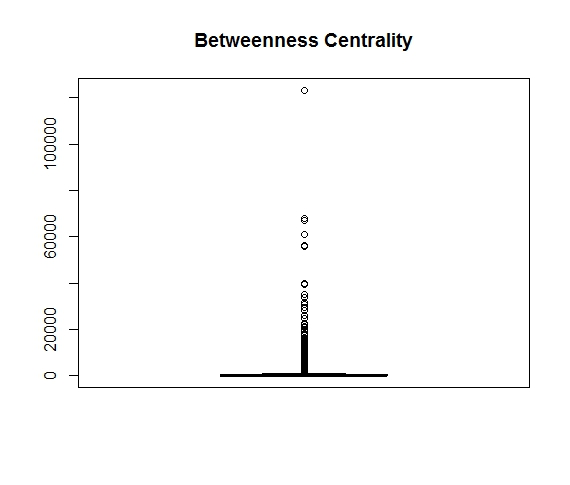
\includegraphics[scale=0.5]{Images/plot_between.jpeg}
%\end{center} 
%\vspace{2mm}  

Words with the highest betweenness scores are as follows:  result (123287.95), use (67756.22), model (67159.62), data (60749.09), suggest (56224.20), and studi (55947.48). As predicted, these words are used often in each document no matter what discipline the document is in. The concept of TopicMapping is successful in this network due to the fact that words from one topic (i.e. one journal) tend to cluster, while very few words tend to act as bridges between these clusters. In fact, out of the $2259$ words in the network, only $758$ have a betweenness centrality greater than one, while $1774$ have a betweenness score greater than $0$. Next, I will find the transitivity score of the network. Due to the clustering of the nodes, I hypothesis that this value is positive and high. In fact it is $0.4081$, with the following triad census:
	\vspace{2mm}
	\begin{center}
		\begin{tabular}{ ||c|c|c|c|c|c|c|c|c|c|c|c|c|c|c|c||  }
			\hline
			 003&012&102&021D&021U&021C&111D&111U&030T&030C&201&120D \\ 
			\hline 
			1610184416&0&282643927&0&0&0&0&0&0&0&21085290&0\\
			\hline
		\end{tabular}
	\end{center}
	\begin{flushleft}
		\begin{tabular}{||c|c|c|c||}
			\hline
			120U&120C&210&300\\
			\hline
			0&0&0&4845576 \\
			\hline
		\end{tabular}
	\end{flushleft}
	\vspace{2mm}
\noindent We can see that the transitivity is in fact positive and moderately high. We also notice that the only triads to form are $003, 102, 201,$ and $300.$ Since this is an undirected graph, these triads are not surprising. The majority of triads $83.9\%$ are in group $003$, where no words are connected, $14.7\%$ are in group $102,$ where two words are connected and neither are connected to the third, $1\%$ are in group $201$, where one word is connected to both of the other words that are not connected to each other, and $0.2\%$ are in $300,$ where all three words are connected. Lastly, I found that the degree assortitivity is positive and low at $0.0149$. Here we see that words which are highly connected do not tend to connect with each other. 
  
\newpage
\section{Bibliography}
\begin{thebibliography}{4}

	\bibitem{lda}
	Blei, D., Ng, A., and Jordan, M.  (2003),
	``Latent Dirichlet Allocation."
	\textit{Journal of Machine Learning Research}: 3 993-1022.
	
	\bibitem{plsa}
	BHoffman, T.  (1999),
	``Probabilistic Latent Semantic Indexing."
	\textit{Proccedings of the Twenty-Second Annual International SIGIR Conferance}.
	
	\bibitem{main}
	Lancichinetti, A., Sirer, M., Wang, J., Acuna, D., Kording, K., and Amaral, Luis. (2015),
	``High-Reproducibility and High-Accuracy Method for Automated Topic Classification."
	\textit{Physical Review X}: 5, 0011007, 2160-3308.
	
	\bibitem{mainExtra}
	Lancichinetti, A., Sirer, M., Wang, J., Acuna, D., Kording, K., and Amaral, Luis. (2015),
	``High-Reproducibility and High-Accuracy Method for Automated Topic Classification: Supplemental Material."
	\textit{Physical Review X}: 5, 0011007, 2160-3308.
	
\end{thebibliography}
	
	
	
\end{document}